\documentclass{article}
\usepackage[top=2cm,bottom=2cm,left=2cm,right=3.5cm]{geometry}
\usepackage{pgfplots}
\usepackage{graphicx}
\usepackage{subcaption}
\usepackage{tikz}

\pgfplotsset{
    every axis/.style={
        width=0.65\textwidth,
        height=6cm,
        ymin=0,
        ylabel={Time (ms)},
        xlabel={Algorithm},
        xtick=data,
        grid=major,
        legend pos=north west,
        major grid style={line width=.1pt,draw=gray!30},
        xticklabels={Thread-row,Warp-row,Shared-mem,Block-row},
    }
}
\pgfplotsset{compat=1.18}

\usepackage[utf8]{inputenc}
\usepackage[most]{tcolorbox}
\tcbuselibrary{skins,breakable}

\newtcolorbox{callout}[2][]{breakable,sharp corners, skin=enhancedmiddle jigsaw,parbox=false,
boxrule=0mm,leftrule=2mm,boxsep=0mm,arc=0mm,outer arc=0mm,attach title to upper,
after title={.\ }, coltitle=purple,colback=purple!10,colframe=purple, title={#2},
fonttitle=\bfseries,#1}

\newtcolorbox{warning}[2][]{breakable,sharp corners, skin=enhancedmiddle jigsaw,parbox=false,
boxrule=0mm,leftrule=2mm,boxsep=0mm,arc=0mm,outer arc=0mm,attach title to upper,
after title={!\ }, coltitle=red,colback=red!10,colframe=red, title={#2},
fonttitle=\bfseries,#1}

\newtcolorbox{esempio}[2][]{breakable,sharp corners, skin=enhancedmiddle jigsaw,parbox=false,
boxrule=0mm,leftrule=2mm,boxsep=0mm,arc=0mm,outer arc=0mm,attach title to upper,
after title={:\ }, coltitle=blue,colback=blue!10,colframe=blue, title={#2},
fonttitle=\bfseries,#1}


\usepackage[parfill]{parskip}
\hypersetup{
    colorlinks=true,
    linkcolor=black,
    % filecolor=magenta,      
    urlcolor=blue,
    % pdftitle={Overleaf Example},
    % pdfpagemode=FullScreen,
}

\usepackage{graphicx}
\usepackage{algorithm2e}

\title{
    GPU computing homework\\
\large CSR group}
\author{Diego Oniarti - 257835 \\ diego.oniarti@studenti.unitn.it \\ \url{https://github.com/diego-oniarti/GPU_homework}}
\date{}

\begin{document}

\maketitle

\section{Problem description and algorithm}
The problem at hand is that of performing a \textit{Sparse-Matrix Dense-Vector Multiplication}.\\The program will receive a sparse matrix, convert it in CSR form, and then multiply it with a dense vector filled with random values.

Beside a sequential CPU implementation 3 different GPU kernels have been implemented:
\begin{enumerate}
    \item \textbf{1 Thread Per Row}: This implementation improves on the sequential one by assigning one thread for each row of the matrix. This thread iterates linearly through the row, multiplying the values by the ones in the vector and summing them together. The output is then saved to an output vector.
    \item \textbf{1 Warp Per Row}: An improvement on the previous implementation, where each row gets an entire warp of threads instead of a single one.\\
        The threads in a warp iterate through the row with stride equal to the warp size and store the partial result in a buffer. These partial results are then summed together by a reduction, and the first thread in the warp with the lowest id stores the final result in the result vector.
    \item \textbf{1 Warp Per Row with Shared Memory} This final implementation works like the previous one, but instead of storing the partial results in a buffer array, they're stored in shared memory.
\end{enumerate}
One more improvement would be to assign a single thread to each nonzero value of the matrix. Implementing this solution makes it hard to sum the values in a row, since there occasionally needs to be a sum between values processed by threads in different blocks, and synchronization becomes cumbersome.

\SetAlgoVlined
\begin{algorithm}[!ht]
    \caption{Warp Per Row}
    \Input{data\_t *vals, *vec, *ret, *buffer,\\
    int *xs, *ys, cols, rows}
    int wid = threadIdx.x / 32\Comment*[r]{Warp id}
    int friend\_id = threadIdx.x \% 32\Comment*[r]{Thread's place in the warp}
    int row = blockIdx.x * (blockDim.x / 32) + wid\Comment*[r]{Row in the matrix}

    buffer[tid] = 0\Comment*{Set to zero to avoid breaking the reduction}
    \If {(row $<$ rows)} {
        int start = ys[row]\;
        int end = ys[row+1]\;

        \Comment{Loop with stride equal to the warp size\\Needed in case there are more elements in a row than threads in a warp}
        data\_t sum = 0\;
        \For {(int i=start+friend\_id; i$<$end; i+=32)} {
            sum += vals[i] * vec[xs[i]]\;
        }
        buffer[tid] = sum\;
    }

    \Comment{Perform the reduction over the warp}
    \For {(int s=1; s$<$32; s$<<=$1)} {
        \_\_syncthreads() \Comment*[r]{Wait for the previous iteration to be over}
        \If {((tid $\&$ ((s$<<$1)-1)) == 0)} {
            buffer[tid] += buffer[tid+s]\;
        }
    }

    \Comment{The first thread in the warp is tasked with moving the result to the output}
    \If {(friend\_id==0 $\&\&$ row$<$rows)} {
        ret[row] = buffer[tid];
    }
\end{algorithm}

\section{Experimental setup}
% \begin{center}
%     \begin{tabular}{|l|l|}
%         \hline
%         Device Name & NVIDIA A30 \\ \hline
%         Memory Clock Rate & 1215.0 MHz \\ \hline
%         Memory Bus Width & 3072 bits \\ \hline
%         Theoretical Memory Bandwidth & 933.12 GB/s \\ \hline
%     \end{tabular}
% \end{center}
The code has been ran on an NVIDIA A30 with 1215 MHz of memory clock rate and a memory bus width of 3072 bits. This puts the theoretical memory bandwidth at $clockrate \cdot bus\ width \cdot 2 = 933.12$ GB/s.

Each algorithm has been ran 13 times, 3 of which being pre-runs and 10 being actual timed runs.\\
The algorithms have been tested with different block sizes, ranging from 32 to 1024.\\
The tests have been performed on a random uniform matrix and 3 matrices sourced from the \href{https://sparse.tamu.edu/}{SuiteSparse Matrix Collection}.
\begin{center}
    \begin{tabular}{l|r|r|rl|l}
        name & rows & columns & nonzeros & (\%) & type \\
        \hline
        lp\_ganges\footnotemark & 1309 & 1706 & 6937 & 0.3106\% & real \\
        delaunay\_n23\footnotemark & 8388608 & 8388608 & 50331568 & 7.152546e-5\% & binary \\
        Stanford\_Berkeley\footnotemark & 683446 & 683446 & 7583376 & 0.001624\% & binary \\
        random & 30000 & 20000 & 6001585 & 1.000264\% & real \\
    \end{tabular}
\end{center}
\footnotetext[1]{\url{https://www.cise.ufl.edu/research/sparse/matrices/LPnetlib/lp_ganges}}
\footnotetext[2]{\url{https://www.cise.ufl.edu/research/sparse/matrices/DIMACS10/delaunay_n23}}
\footnotetext[3]{\url{https://www.cise.ufl.edu/research/sparse/matrices/Kamvar/Stanford_Berkeley}}

\section{Results}

\begin{figure}[!ht]
    \centering
    \begin{subfigure}[t]{0.5\textwidth}
        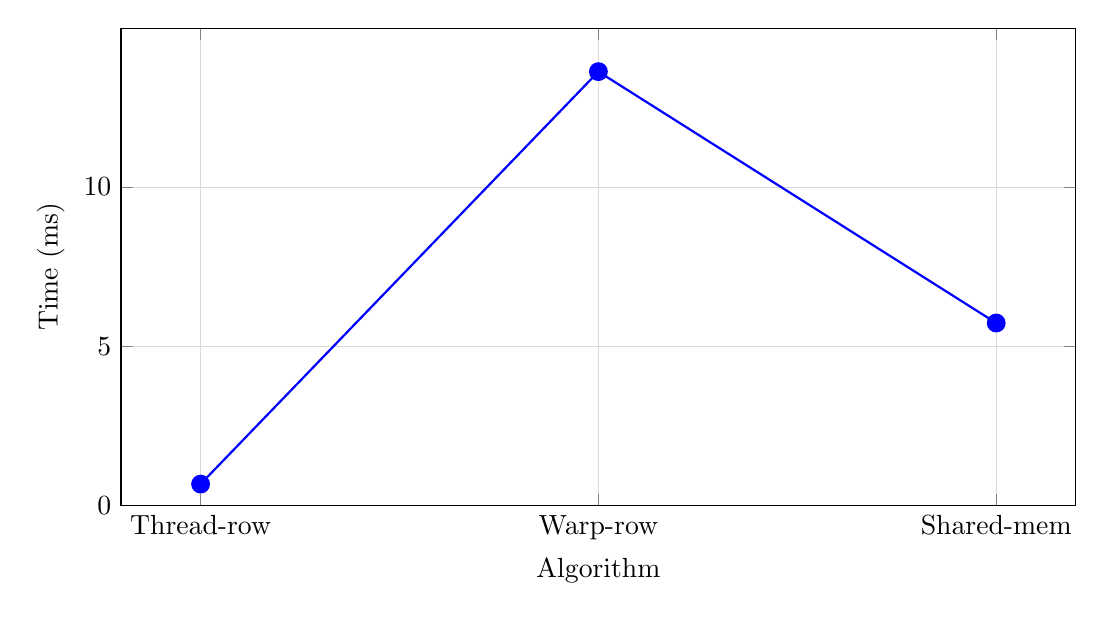
\begin{tikzpicture}
            \begin{axis}[
                width=\textwidth,
                height=0.5\textwidth,
                scale only axis,
                every axis plot/.append style={thick}
            ]
                \addplot[blue,mark=*,mark size=3pt] coordinates {
                    (1, 0.676)
                    (2, 13.624)
                    (3, 5.732)
                };
            \end{axis}
        \end{tikzpicture}
    \end{subfigure}%
    \hfill% Add space between subfigures
    \begin{subfigure}[t]{0.4\textwidth}  % Total width now 0.7 + 0.28 ≈ 1.0
        \raisebox{0.4cm}{
            \includegraphics[width=\textwidth,trim=1.8cm 0 0 0,clip]{images/delaunay_n23.png}
        }
    \end{subfigure}%
    \caption{delaunay\_n23}%
    \label{fig:delaunay}
\end{figure}

\begin{figure}[!ht]
    \centering
    \begin{subfigure}[t]{0.5\textwidth}
        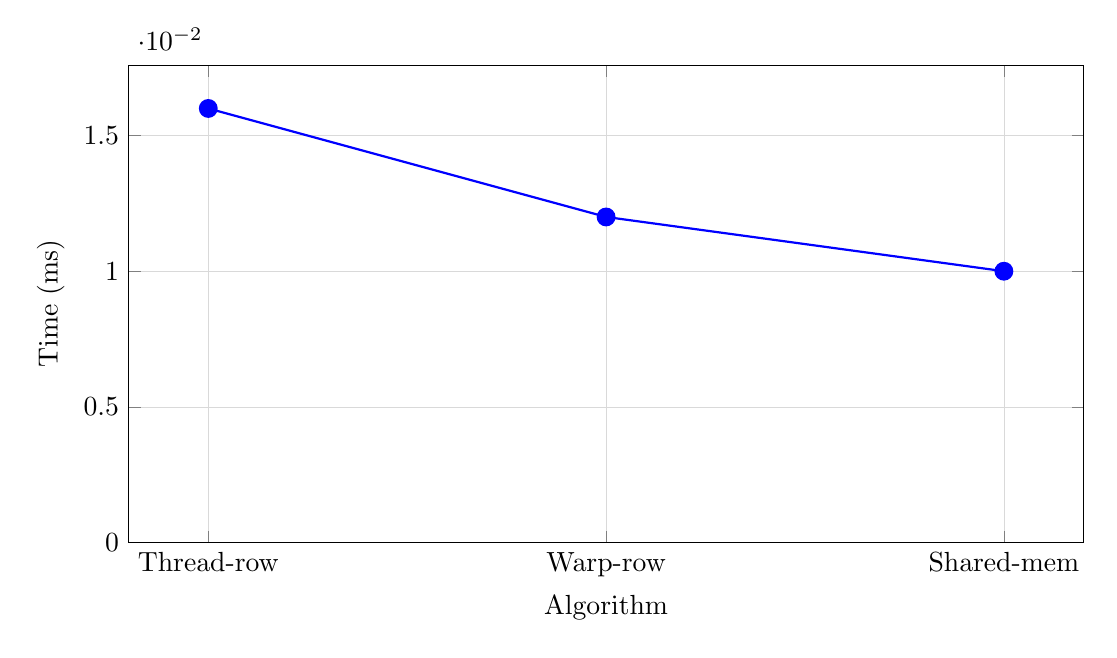
\begin{tikzpicture}
            \begin{axis}[
                width=\textwidth,
                height=0.5\textwidth,
                scale only axis,
                every axis plot/.append style={thick}
            ]
                \addplot[blue,mark=*,mark size=3pt] coordinates {
                    (1,0.016)
                    (2,0.012)
                    (3,0.01)
                };
            \end{axis}
        \end{tikzpicture}
    \end{subfigure}%
    \hfill% Add space between subfigures
    \begin{subfigure}[t]{0.4\textwidth}  % Total width now 0.7 + 0.28 ≈ 1.0
        \raisebox{0.4cm}{
            \includegraphics[width=\textwidth,trim=1.8cm 0 0 0,clip]{images/lp_ganges.png}
        }
    \end{subfigure}%
    \caption{lp\_ganges}%
    \label{fig:ganges}
\end{figure}

\begin{figure}[!ht]
    \centering
    \begin{subfigure}[t]{0.5\textwidth}
        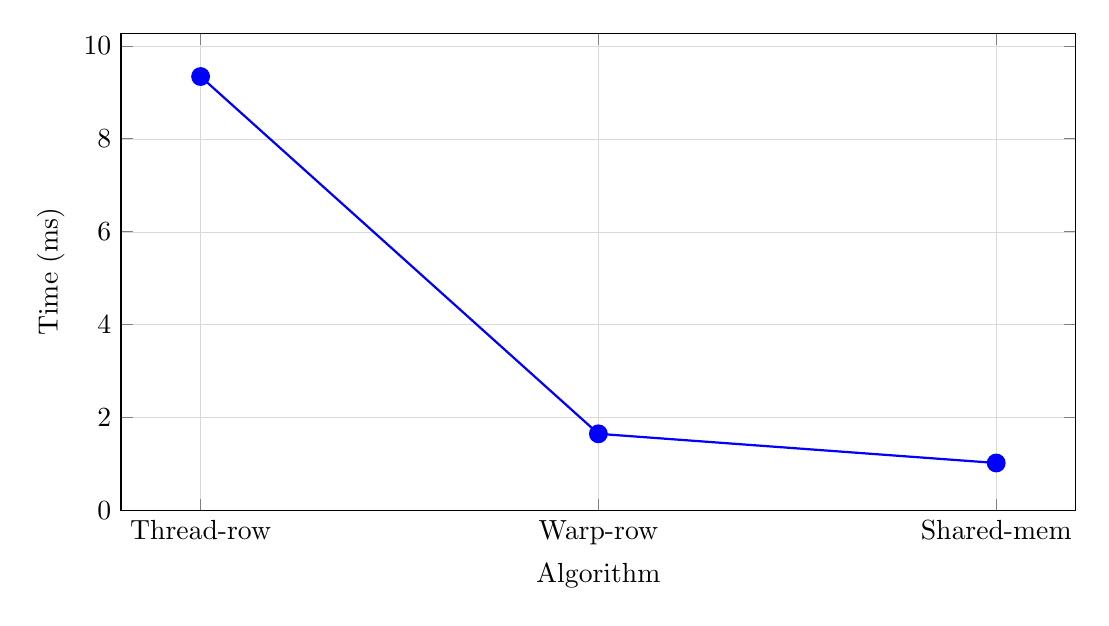
\begin{tikzpicture}
            \begin{axis}[
                width=\textwidth,
                height=0.5\textwidth,
                scale only axis,
                every axis plot/.append style={thick}
            ]
                \addplot[blue,mark=*,mark size=3pt] coordinates {
                    (1,9.339)
                    (2,1.65)
                    (3,1.022)
                };
            \end{axis}
        \end{tikzpicture}
    \end{subfigure}%
    \hfill% Add space between subfigures
    \begin{subfigure}[t]{0.4\textwidth}  % Total width now 0.7 + 0.28 ≈ 1.0
        \raisebox{0.4cm}{
            \includegraphics[width=\textwidth,trim=1.8cm 0 0 0,clip]{images/Stanford_Berkeley.png}
        }
    \end{subfigure}%
    \caption{Stanford\_Berkley}%
    \label{fig:stanford}
\end{figure}

\begin{figure}[!ht]
    \centering
    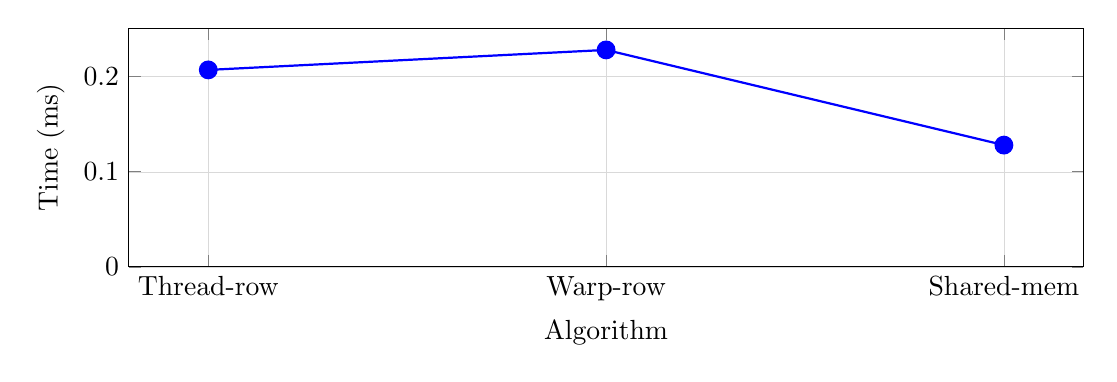
\begin{tikzpicture}
        \begin{axis}[
            width=\textwidth,
            height=0.25\textwidth,
            scale only axis,
            every axis plot/.append style={thick}
            ]
            \addplot[blue,mark=*,mark size=3pt] coordinates {
                    (1,0.207)
                    (2,0.228)
                    (3,0.128)
                };
        \end{axis}
    \end{tikzpicture}
    \caption{Uniform random matrix}%
    \label{fig:random}
\end{figure}

\begin{figure}[!ht]
    \centering
    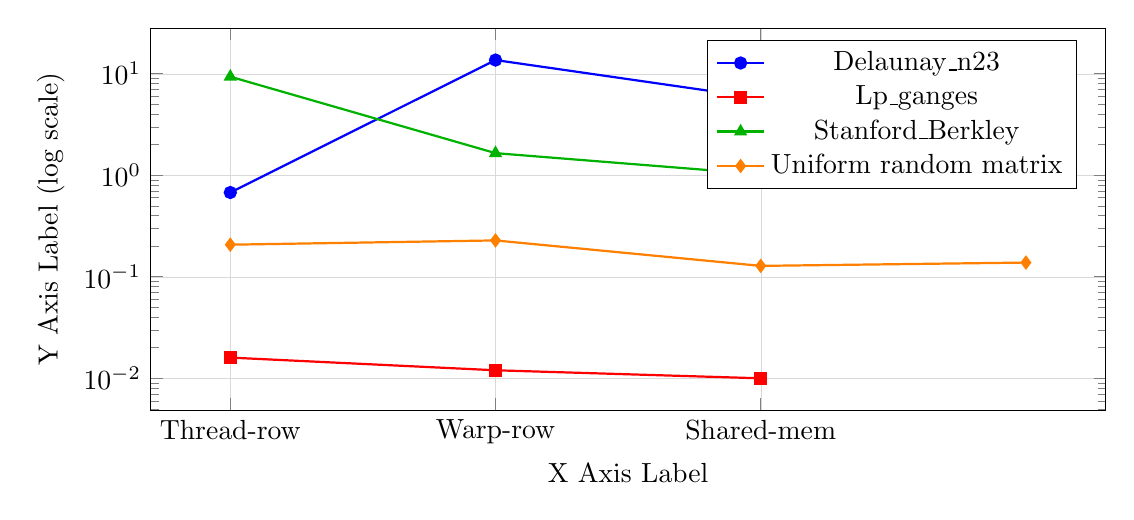
\begin{tikzpicture}
        \begin{axis}[
            width=\textwidth,
            height=0.4\textwidth, % Increased height for better visibility
            scale only axis,
            ymode=log, % Logarithmic Y-axis
            legend pos=north east,
            grid=major, % Optional grid
            xlabel={X Axis Label}, % Add your X-axis label
            ylabel={Y Axis Label (log scale)}, % Add your Y-axis label
            cycle list={ % Custom cycle list for colors and markers
                blue,mark=*\\ % Dataset 1
                red,mark=square*\\ % Dataset 2
                green!70!black,mark=triangle*\\ % Dataset 3
                orange,mark=diamond*\\ % Dataset 4
            },
            every axis plot/.append style={thick},
            ]
            
            % Dataset 1 (original example)
            \addplot+[mark size=2pt] coordinates {
                    (1, 0.676)
                    (2, 13.624)
                    (3, 5.732)
            };
            \addlegendentry{Delaunay\_n23}

            % Dataset 2 (example with higher values)
            \addplot+[mark size=2pt] coordinates {
                    (1,0.016)
                    (2,0.012)
                    (3,0.01)
            };
            \addlegendentry{Lp\_ganges}

            % Dataset 3 (another example)
            \addplot+[mark size=2pt] coordinates {
                    (1,9.339)
                    (2,1.65)
                    (3,1.022)
            };
            \addlegendentry{Stanford\_Berkley}

            % Dataset 4 (another example)
            \addplot+[mark size=2pt] coordinates {
                    (1,0.207)
                    (2,0.228)
                    (3,0.128)
                    (4,0.138)
            };
            \addlegendentry{Uniform random matrix}

        \end{axis}
    \end{tikzpicture}
    \caption{Combined data series on logarithmic scale}%
    \label{fig:combined_plot}
\end{figure}
\end{document}


